\documentclass[12pt,a4paper]{article}
\usepackage[a4paper,margin=1in]{geometry}
\usepackage[T1]{fontenc}
\usepackage{lmodern}
\usepackage{amsmath,amssymb}
\usepackage{graphicx}
\usepackage{booktabs}
\usepackage{array}
\usepackage{enumitem}
\usepackage[hidelinks]{hyperref}
\usepackage{url}
\usepackage{setspace}
\setstretch{1.1}
\setlength{\parskip}{5pt}
\setlength{\parindent}{0pt}
\setcounter{tocdepth}{2}

\begin{document}

%================ COVER PAGE ================
\begin{titlepage}
\centering
\vspace*{1.5cm}
{\LARGE\bfseries FedQPNT: Attack-Resilient Vehicle Navigation with Quantum Inertial Aiding, Federated Attack Detection and Continuous GNSS Trust\par}
\vspace{1.5cm}
{\Large\bfseries Review 3 Report\par}
\vspace{1.5cm}
{\large Project basket: Novelty project (journal paper draft + patent claim draft)\par}
\vspace{2cm}
\begin{tabular}{rl}
\textbf{Team name:} & [Team name]\\[6pt]
\textbf{Members:} & [Member names and register numbers]\\[6pt]
\textbf{Guide:} & [Guide: Professor name]\\[6pt]
\textbf{Course / Slot:} & [Course code / Slot]\\[6pt]
\textbf{Department:} & [Department, University]
\end{tabular}
\vfill
{\large October 2026\par}
\end{titlepage}

%================ ABSTRACT ================
\pagenumbering{roman}
\section*{Abstract}
\addcontentsline{toc}{section}{Abstract}
Global Navigation Satellite System (GNSS) spoofing and jamming threaten autonomous vehicles and unmanned aerial vehicles. We present FedQPNT, which fuses an inertial measurement unit, GNSS and a cold-atom accelerometer (CAI) in an error-state Kalman filter. A learned detector drives a continuous, asymmetric trust law with evidence-bounded exclusion, and detector parameters are aggregated across a fleet by a robust federated-learning (FL) aggregator. The CAI noise model is calibrated to real laboratory data; platform, GNSS observables and attacks are simulated. We report a pre-registered evaluation on 30 unseen seeds per scenario at two inertial grades, with a Holm-corrected confirmatory family of eight tests. FedQPNT detects attack onset significantly earlier than a detect-and-exclude baseline (median paired difference 0.5\,s, Holm-adjusted $p=0.004$); the accompanying position-error test was not significant. It adds no measurable cost in nominal operation or under jamming. Against a displaced meaconer it lowers attack-window horizontal error relative to the baseline at both grades and to the undefended filter at the MEMS grade, and it cuts median clock error about eight-fold (634 versus 5220\,ns). Trust cycling stayed at or below 29 cycles per hour (proven bound: 223), and a four-hour mission showed no drift. The evaluation also characterises where GNSS exclusion does not pay: for small-offset spoofs an inertial coast drifts further than the spoof displaces, and the re-admission dwell dominates post-attack error. The CAI and federated learning showed no measurable effect in this configuration (hypotheses H2--H4 not supported).

\newpage
\tableofcontents
\newpage
\pagenumbering{arabic}

%=====================================================================
\section{Introduction}
%=====================================================================

\subsection{Motivation}
Positioning, navigation and timing (PNT) for autonomous vehicles and UAVs depends heavily on GNSS, a signal that is inexpensive to spoof or jam and whose loss or manipulation directly threatens safety. In plain terms, a spoofer broadcasts a fake satellite signal so that the receiver believes it is somewhere else, or at another time; a jammer drowns the real signal in noise. A vehicle that trusts GNSS blindly follows the fake signal, while a vehicle that distrusts it too readily must navigate on inertial sensors alone, whose error grows with time.

A wide literature addresses parts of this problem: federated learning has been used to detect GNSS spoofing across a fleet without centralizing raw sensor data \cite{khan2025enhancing,chai2025navigation,liu2026g2fl,namagembe2026machine,zhou2023spatiotemporal}; classical and learned adaptive filters re-weight or exclude GNSS when it disagrees with inertial propagation \cite{mehra1970identification,carlson1988federated,carlson1990federated,ren2020adaptive,pardhasaradhi2022gps,negru2024resilient}; and cold-atom interferometers (CAIs) have been proposed and increasingly demonstrated as inertial sensors whose bias is orders of magnitude below that of classical accelerometers \cite{wright2022cold,darmagnac2024atom}. Separately, quantum-enhanced and quantum federated learning have been studied as a way to speed up or secure the \emph{learning computation} itself \cite{hazarika2025quantum,chehimi2023foundations,chehimi2022quantum}. To date, however, these threads have not been combined: no verified prior work couples (a) a physical quantum inertial sensor, (b) fleet-wide federated learning of an attack detector, and (c) a continuous, attack-adaptive trust law that keeps this detector's output as a smoothly varying confidence rather than a switch.

\subsection{Problem statement and gap}
\label{sec:gap}
No verified reference in our bibliography (Section~\ref{sec:related}, Table~\ref{tab:comparison}) implements federated learning together with a physical quantum inertial sensor, and among the FL-based GNSS-defense papers we could verify, all use a binary detect-and-exclude action rather than a continuously varying trust weight. Conversely, the continuous/adaptive-trust literature either has no federated learning component or, when described as ``federated'', uses the classical multi-sensor ``federated filter'' sense of the term (master/local filter fusion within one platform) \cite{negru2024resilient}. The specific, scoped gap addressed is therefore: \emph{a closed loop in which an FL-trained, fleet-shared spoofing/jamming detector drives a continuous, evidence-bounded, per-sensor trust weight that gates a quantum-aided navigation filter, with the quantum sensor's own noise and fault behaviour calibrated to real laboratory data rather than assumed.}

\subsection{Objectives}
The project has four objectives, each stated as a falsifiable hypothesis before any test result was seen (Section~\ref{sec:hypotheses}):
\begin{itemize}[nosep]
\item H1: continuous trust improves on a binary detect-and-exclude baseline (Baseline~A) in attack-window position error and detection latency;
\item H2: fleet-shared learning improves on single-node learning for an attack family the node has not experienced;
\item H3: quantum aiding improves detection latency for gradual spoofing;
\item H4: fleet-shared learning improves detection by a cold-start node.
\end{itemize}

\subsection{Contributions}
\begin{itemize}
\item A system architecture in which a single 15-state loosely-coupled error-state Kalman filter is shared, unmodified, across every baseline and ablation, so that comparisons isolate the contribution of each mechanism rather than confounding it with implementation differences (Section~\ref{sec:method}).
\item A continuous, asymmetric trust law with evidence-bounded exclusion (a bounded distrust time, a shadow probe that tests returning GNSS against the coasting state without applying it, and separate position and clock trust weights) that couples a learned, federated detector to the measurement covariances via a bounded inflation $R_{\mathrm{eff}} = R / \max(w, w_{\min})$, with trust cycling bounded at $223$ cycles per hour independently of the timing of the evidence.
\item TRIM-NB-R, a trust-aware robust federated aggregator combining norm clipping, coordinate-wise trimmed-mean/median aggregation, and a cosine-similarity reputation score with quarantine; the round-3 evaluation does not include an AUC-based poisoning comparison, so its robustness benefit is specified but not evaluated here.
\item A quantum inertial sensor model whose noise density, per-interrogation-time noise scaling and bursty fault process are calibrated from real cold-atom interferometer shot data \cite{darmagnac2024atom}, together with an explicitly reported operating limit (rigid-mode contrast loss above $\Omega_c \approx 17\,\mathrm{mrad/s}$).
\item A pre-registered, mechanism-class baseline taxonomy (A: FL detect-and-exclude; B-bin: single-node detect-and-switch; B-cont: single-node continuous trust; B$'$: classical innovation-based adaptive filter) and four hypotheses H1--H4, reported whatever their outcome.
\end{itemize}

\subsection{Report organisation}
Section~\ref{sec:related} surveys related work. Section~\ref{sec:method} gives the threat model, sensor models, fusion filter, detector, trust engine, federated learning and the evaluation protocol. Section~\ref{sec:results} reports the experimental results. Section~\ref{sec:conclusion} concludes with limitations and future work.

%=====================================================================
\section{Related Work}
\label{sec:related}
%=====================================================================

\subsection{Federated learning for GNSS security}
Several recent papers apply federated learning to GNSS spoofing or jamming detection so that a fleet of vehicles can share a detector without centralizing raw trajectory data. Khan et al.\ \cite{khan2025enhancing} have each vehicle localize itself from dead-reckoning-style signals, compare this against GNSS, and aggregate the resulting mismatch-based weights at a roadside unit, where a global support-vector machine is trained by FL; they report 99\% accuracy on CARLA-simulated trajectories. Chai et al.\ \cite{chai2025navigation} similarly use federated learning to identify spoofing and jamming signals for UAVs, and Namagembe et al.\ \cite{namagembe2026machine} propose a machine-learning GPS spoofing detection and mitigation scheme for UAVs. Zhou et al.\ \cite{zhou2023spatiotemporal} propose spatial-temporal federated transfer learning for cooperative positioning, which targets accuracy under heterogeneous data rather than adversarial spoofing. Closest to our robust-aggregation component is G\textsuperscript{2}FL \cite{liu2026g2fl}, a robust FL scheme for GNSS spoofing detection under Byzantine or poisoned clients. In every one of these papers the FL-trained detector's output drives a \emph{binary} decision at the node; none couples the detector to a continuously varying trust weight on the fusion filter's measurement covariance, and none uses a physical quantum sensor.

\subsection{Adaptive and fault-tolerant sensor fusion and trust}
Re-weighting or excluding a sensor based on its own innovation statistics predates federated learning by decades. Mehra \cite{mehra1970identification} introduced innovation-based adaptive estimation for Kalman filters, the basis of our B$'$ baseline. Carlson's federated filter \cite{carlson1988federated,carlson1990federated} decomposes a navigation filter into local filters per sensor feeding a master filter; this is the classical, single-platform sense of ``federated''. Ren et al.\ \cite{ren2020adaptive} demonstrate adaptive fusion of camera, GNSS and IMU for autonomous driving, which we use as the representative of the single-node continuous-weighting class (B-cont). Pardhasaradhi and Cenkeramaddi \cite{pardhasaradhi2022gps} detect GPS spoofing on a drone via distributed radar tracking and switch to the radar track once spoofing is flagged, the representative of our detect-and-switch class (B-bin). Negru et al.\ \cite{negru2024resilient} integrate GNSS, IMU, camera and barometer with local extended Kalman filters feeding a gated-recurrent-unit master filter; despite the word ``federated'' in its title, this is the Carlson-style federated \emph{filter} inside a single UAV, not federated learning across clients. A companion paper \cite{negru2024uwb} studies UWB-aided navigation in degraded GNSS. None of this group's mechanisms is trained or shared across a fleet, and none uses a physical quantum sensor.

\subsection{Quantum inertial sensing for navigation}
Cold-atom interferometers measure acceleration or rotation via atom-interferometric phase, giving an absolute output whose bias is set by atomic constants rather than by the drift of a mechanical proof mass. Wright et al.\ \cite{wright2022cold} review cold-atom inertial sensors for navigation, including dead time, dynamic range and size/weight/power challenges on a moving platform. d'Armagnac de Castanet et al.\ \cite{darmagnac2024atom} report a three-axis hybrid cold-$^{87}$Rb atom interferometer operated at arbitrary orientations and rotation rates, providing per-shot population-ratio residuals at several interrogation times and a measured contrast-versus-rotation-rate law. We use this dataset \cite{darmagnac2024dataset} directly to calibrate our simulated CAI's noise density, its per-interrogation-time scaling and a Gilbert--Elliott bursty-outlier channel. Neither work addresses fleet-wide learning or GNSS attack robustness.

\subsection{Quantum federated learning (distinguished from quantum sensing)}
A separate line of work applies quantum \emph{computation} to the federated learning process itself. Hazarika et al.\ \cite{hazarika2025quantum} propose quantum-enhanced FL for vehicular networks; Chehimi et al.\ \cite{chehimi2023foundations,chehimi2022quantum} lay architectural foundations for quantum FL over quantum networks, including quantum data. These address the learning substrate and communication channel, not inertial or positioning sensors, and none targets GNSS spoofing or jamming. We cite them to pre-empt a mistaken reading of ``quantum federated learning for navigation'' as prior work equivalent to ours.

\subsection{GNSS spoofing and jamming signatures}
Psiaki and Humphreys \cite{psiaki2016gnss} survey spoofing mechanisms and detection, including capture-and-carry-off dynamics and the vulnerability of a receiver at re-acquisition after an outage; Humphreys et al.\ \cite{humphreys2008assessing} assess the practical threat. Radoš et al.\ \cite{rados2024recent} report field-measured signatures we rely on, including the collapse of cross-satellite C/N0 correlation under single-antenna spoofing (from $-0.76$ clean to $0.99$ spoofed). Borhani-Darian et al.\ \cite{borhanidarian2024detecting} classify spoofing from the cross-ambiguity function, a lower, pre-tracking level than our raw-observable level, and Tariq and Ahanger \cite{tariq2026multimodel} fuse Kalman filtering with ensemble and transformer models for BeiDou spoofing across a UAV swarm (about 99\% detection accuracy reported; the often-quoted 97\% figure is a mission-success rate). Together these motivate our attack simulator and detector feature set.

\subsection{Comparison}
Table~\ref{tab:comparison} positions FedQPNT against the verified related systems on the four properties it combines.

\begin{table}[ht]
\centering
\caption{Comparison of related systems. ``FL?'' = detector trained/aggregated across distributed clients (not the single-platform ``federated filter''). ``Quantum?'' = physical quantum sensor (not quantum-enhanced computation). ``Adaptive trust?'' = continuously varying, not binary, trust during an attack. ``Attack-tested?'' = evaluated under an explicit attack scenario in the cited paper.}
\label{tab:comparison}
\footnotesize
\begin{tabular}{p{3.0cm}p{1.8cm}p{2.0cm}p{3.4cm}p{2.3cm}}
\toprule
System / paper & FL? & Physical quantum sensor? & Adaptive (continuous) trust? & Attack-tested? \\
\midrule
Khan et al.\ 2025 \cite{khan2025enhancing} & Yes & No & Not stated (detection only) & Yes (spoofing) \\
Chai et al.\ 2025 \cite{chai2025navigation} & Yes & No & No (classification only) & Yes (spoofing/jamming) \\
G\textsuperscript{2}FL, Liu et al.\ 2026 \cite{liu2026g2fl} & Yes (robust) & No & No & Yes (spoofing, Byzantine) \\
Negru et al.\ 2024 \cite{negru2024resilient} & No (federated \emph{filter}) & No & Continuous (GRU master filter) & No (degraded GNSS) \\
Pardhasaradhi \& Cenkeramaddi 2022 \cite{pardhasaradhi2022gps} & No & No & No (detect-and-switch) & Yes (spoofing) \\
Hazarika et al.\ 2025 \cite{hazarika2025quantum} & Yes & No (quantum compute) & No & No \\
Chehimi et al.\ 2023 \cite{chehimi2023foundations} & Yes (quantum FL) & No & No & No \\
Tariq \& Ahanger 2026 \cite{tariq2026multimodel} & No (multi-model fusion) & No & Partial (ensembling) & Yes (BeiDou spoofing) \\
\textbf{FedQPNT (this work)} & \textbf{Yes} & \textbf{Yes (real-data-calibrated)} & \textbf{Yes (continuous, evidence-bounded exclusion)} & \textbf{Yes (15-scenario matrix)} \\
\bottomrule
\end{tabular}
\end{table}

%=====================================================================
\section{Methodology}
\label{sec:method}
%=====================================================================
This section condenses the specification of the reference simulator. Parameters are tagged by provenance: \emph{measured} (fitted to the real cold-atom data of \cite{darmagnac2024atom}), \emph{datasheet}, or \emph{assumed} (a design value that is swept or stress-tested rather than claimed).

\subsection{System and threat model}
\label{sec:threat}
The system is a fleet of $N$ independent nodes (ground vehicles or UAVs) running the same code. Every node is split into an \emph{Environment} half (ground-truth trajectory, sensor models, GNSS signal generation and attacks) and an \emph{Agent} half (GNSS receiver, fusion filter, trust engine, learnable detector and FL client). Only sensor outputs cross from Environment to Agent; ground truth and the per-tick attack label never do, enforced by construction and by an automated static-analysis guard. A node runs a 100~Hz global tick. Nodes exchange only federated-learning model updates with a server on a fixed round schedule; navigation never blocks on a fresh global model, so a node that has lost communications keeps navigating with its last detector.

The attacker acts only on the GNSS signal, at the raw-observable level (per-satellite pseudorange, pseudorange rate, C/N0, lock state, AGC), never on the IMU, the quantum sensor or the inter-node channel. Five attack families are modelled: (i) gradual (``drift-in'') spoofing, in which a single-antenna spoofer captures the tracking loops and drags the measurements toward a fake trajectory; (ii) meaconing (record-and-rebroadcast), a common-mode clock/delay shift across all satellites; (iii) abrupt spoofing, which forces a loss of lock and a position jump on re-lock; (iv) continuous-wave and wideband jamming; and (v) combined jam-then-spoof, the classic window in which a receiver is most vulnerable \cite{psiaki2016gnss}. The single-antenna signature (common-mode C/N0 fluctuation, loss of elevation dependence) follows field statistics \cite{rados2024recent}. In the FL threat surface a fraction $f$ of nodes may be Byzantine (sign-flip, Gaussian, label-flip or ``A Little Is Enough'' updates); the self-reported sample count is untrusted.

No raw sensor stream, trajectory or attack label ever leaves a node. The only object sent to the server is a \texttt{ModelUpdate}: a detector weight delta (1010 parameters, about 4~kB), feature-normalisation statistics and scalar training metrics. Trust-law hyperparameters and the filter are fixed, identical across all compared methods, and tuned once on disjoint tuning seeds before any test result was examined.

\subsection{Sensor models}
\label{sec:sensors}
\paragraph{Classical IMU.}
Each axis follows an IEEE Std~952-style error budget \cite{ieee952}: constant turn-on bias, a first-order Gauss--Markov bias-instability process, white noise, scale-factor and misalignment errors, quantisation and saturation (GM1 standard deviation $\sigma_{\mathrm{GM}} = B/0.664$ \cite{jurado2019regression}). Two grades are reported separately (Table~\ref{tab:imu}), following ADIS16470-class and HG1700-class parts \cite{adi2017adis16470,honeywell2025hg1700}.

\begin{table}[ht]
\centering
\caption{IMU grades. ``D'' = datasheet figure, ``A'' = assumed. Both run at $100\,\mathrm{Hz}$.}
\label{tab:imu}
\small
\begin{tabular}{lcc}
\toprule
Parameter & Industrial MEMS & Tactical \\
\midrule
Gyro in-run bias stability & 8$^\circ$/h (D) & 1$^\circ$/h (D) \\
Gyro angular random walk & 0.34$^\circ/\sqrt{\mathrm{h}}$ (D) & 0.125$^\circ/\sqrt{\mathrm{h}}$ (D) \\
Accel in-run bias stability & 13\,$\mu$g (D) & 30\,$\mu$g (A) \\
Accel white-noise density & 25\,$\mu$g/$\sqrt{\mathrm{Hz}}$ (A) & 15\,$\mu$g/$\sqrt{\mathrm{Hz}}$ (A) \\
Bias correlation time $\tau_c$ & 200\,s (A) & 300\,s (A) \\
Accel turn-on bias & 10\,mg (A) & 2\,mg (A) \\
Gyro turn-on bias & 0.1$^\circ$/s (A) & 0.01$^\circ$/s (A) \\
Scale factor / misalignment & 500\,ppm / 0.3\,mrad (A) & 100\,ppm / 0.1\,mrad (A) \\
\bottomrule
\end{tabular}
\end{table}

\paragraph{GNSS receiver.}
A synthetic Walker-like GPS almanac with a $10^\circ$ elevation mask gives eight to nine visible satellites. Per satellite the simulator generates pseudorange, pseudorange rate, C/N0 (38 to 48\,dB\,Hz from low elevation to zenith, assumed) and AGC. The pseudorange error combines code thermal noise, a Gauss--Markov ionospheric residual, tropospheric delay and multipath \cite{kaplan2017understanding}. A position/velocity/clock fix is solved by weighted least squares \cite{misra2006global} followed by a snapshot residual-based RAIM statistic \cite{pullen2020gnss}, at $1\,\mathrm{Hz}$ by default.

\paragraph{Cold-atom accelerometer (CAI).}
The CAI is a Mach--Zehnder light-pulse interferometer with phase $\phi = k_{\mathrm{eff}}\,a\,T^2$, $k_{\mathrm{eff}} = 1.61\times10^{7}\,\mathrm{rad/m}$ for $^{87}$Rb. The fringe is observed modulo $2\pi$, so the model resolves the fringe order with a classical companion accelerometer as in hybrid matter-wave/classical sensors \cite{cheiney2018navigation,templier2022tracking,wright2022cold}. The primary (FIELD) grade is anchored to real shot data \cite{darmagnac2024atom,darmagnac2024dataset} through four fitted elements (Table~\ref{tab:cai}): a robust per-shot noise $\sigma_{\mathrm{shot}} = 5.60\,\mu g$ at $2T = 20\,\mathrm{ms}$ (bootstrap 95\% CI $[5.04, 6.40]\,\mu g$, $n=491$ shots), interpolated across interrogation times and deliberately not scaled as $1/T^2$; a two-state Gilbert--Elliott bursty-outlier channel with $9.0\%$ outlier probability and $65.9\%$ persistence ($7.4\times$ more adjacency than independence); a contrast loss $C = C_0\exp(-(\Omega_\perp/\Omega_c)^2)$ with $C_0 = 0.394$, $\Omega_c = 48.2\,\mathrm{mrad/s}$ at $2T=12\,\mathrm{ms}$, scaled as $1/T^2$ to $17.3\,\mathrm{mrad/s}$ at $T=10\,\mathrm{ms}$ (physics-derived, unverified away from the measured point); and a cycle time of $1.548\,\mathrm{s}$. The sample is \emph{not} flagged invalid during an outlier burst: the sensor is silently wrong, as a real instrument would be, so the trust engine, not a validity flag, must catch it.

\begin{table}[ht]
\centering
\caption{CAI FIELD-grade parameters. M = measured from \cite{darmagnac2024atom,darmagnac2024dataset}, A = assumed.}
\label{tab:cai}
\small
\begin{tabular}{lcc}
\toprule
Quantity & Value & Basis \\
\midrule
Interrogation time $2T$ & 20\,ms & M \\
Cycle time & 1.548\,s & M \\
Shot noise $\sigma_{\mathrm{shot}}$ & 5.60\,$\mu$g & M \\
Outlier rate / persistence & 9.0\% / 65.9\% & M \\
Contrast $C_0$, $\Omega_c$ ($T{=}6$\,ms) & 0.394, 48.2\,mrad/s & M \\
$\Omega_c$ at $T{=}10$\,ms & 17.3\,mrad/s & $1/T^2$ scaling \\
Contrast threshold; range & 0.08; $2g$ & A \\
Slow bias residual (GM1) & 3\,$\mu$g, $\tau_c{=}300$\,s & A \\
\bottomrule
\end{tabular}
\end{table}

\subsection{Fusion filter}
\label{sec:fusion}
All methods share one loosely coupled 15-state error-state extended Kalman filter (ESKF) with error state $\delta x = [\delta p,\ \delta v,\ \psi,\ \delta b_a,\ \delta b_g]\in\mathbb R^{15}$ \cite{sola2017quaternion}. Process noise follows the IMU configuration. The initial roll/pitch uncertainty is
\begin{equation}
\sigma_{\mathrm{tilt}} = \max\!\big(1\,\mathrm{mrad},\ \sigma_{b_a,0}/g\big),
\label{eq:tilt0}
\end{equation}
since an accelerometer turn-on bias tilts the levelling by about $\sigma_{b_a,0}/g$. The covariance propagation also carries the second moment of the neglected second-order attitude term $d_2 = \tfrac12\,\psi\times(\psi\times f_n)$, a one-signed vertical velocity error growing with tilt squared; without it the coast covariance is over-confident and returning GNSS is never re-admitted. The term has no tuning constant and is part of the shared core.

\paragraph{GNSS update.}
The fix enters as a six-dimensional position/velocity update with
\begin{equation}
R_{\mathrm{g}} = \kappa_R\,\mathrm{blkdiag}\big(\Sigma_{p}^{\mathrm{fix}},\ \Sigma_{v}^{\mathrm{fix}}\big),\qquad \kappa_R = 60,
\label{eq:rgnss}
\end{equation}
where $\kappa_R$ compensates the time-correlated error (ionosphere, troposphere, multipath) that a loosely coupled fix treats as white. It is set once on tuning seeds, identically for every method, so that nominal horizontal ANEES is close to one.

\paragraph{CAI update.}
The CAI enters as a direct observation of the classical accelerometer bias: over the sample's response window the innovation $\nu_{\mathrm{q}} = \bar f_{\mathrm{Q}} - \bar f_{\mathrm{IMU}}\approx \delta b_a + (\text{CAI noise})$, in which gravity, attitude and trajectory cancel, with
\begin{equation}
R_{\mathrm{q}} = \mathrm{diag}(\sigma_{\mathrm{shot}}^2) + \frac{\mathrm{VRW}^2}{T_W}\,I + \sigma_{\mathrm{win}}^2 I,\qquad \sigma_{\mathrm{win}}=10^{-5}g\ \text{(assumed)}.
\label{eq:rq}
\end{equation}

\paragraph{Trust coupling and gating.}
For a sensor $s$ with trust weight $w_s\in[w_{\min},1]$, trust enters only through the effective covariance and an exclusion rule,
\begin{equation}
R_{\mathrm{eff},s} = \frac{R_s}{\max(w_s,\,w_{\min})},\qquad \text{skip the update if } w_s < w_{\mathrm{excl}},
\label{eq:reff}
\end{equation}
with $w_{\min}=0.02$, $w_{\mathrm{excl}}=0.05$ (assumed). A $\chi^2$ gate at level $10^{-4}$ is part of the shared core and is applied \emph{softly}: an update whose normalised innovation squared exceeds the gate has its covariance scaled so its effective NIS equals the gate (a Huber-type robust update), because a hard gate drops a slowly dragged fix once it leaves the $\chi^2$ region, after which inertial coasting diverges. Only the deliberately gate-free ``undefended'' reference lacks the gate.

\paragraph{Clock filter.}
Timing is estimated by a standalone two-state Kalman filter on clock bias and drift, with TCXO oscillator spectral densities $q_b = \tfrac12 c^2 h_0\approx 9.0\times10^{-3}\,\mathrm{m^2/s}$ and $q_d = 2\pi^2 c^2 h_{-2}\approx3.6\times10^{-2}\,(\mathrm{m/s})^2/\mathrm{s}$ \cite{brown2012introduction,krawinkel2021improved,qin2021benefits}. The filter is aided by the fix's clock estimates, with trust applied as in Eq.~\eqref{eq:reff} through a separate clock weight $w_{\mathrm{clk}}$; below $w_{\mathrm{excl}}$ it holds over on the oscillator model. The simulated truth clock uses the same TCXO values, so the timing results are model-consistent by construction.

\subsection{Learned detector}
\label{sec:detector}
At each GNSS epoch a causal extractor produces a 15-dimensional feature vector from the fix and the filter's \emph{nominal-$R$} pre-correction innovations (so a feature cannot depend on its own trust output): position and velocity NIS per degree of freedom, the RAIM statistic, mean C/N0 and its cross-satellite spread, C/N0 rate, AGC, clock-bias and clock-drift jumps against a constant-drift prediction, WLS residual rms, change in satellite count, a Page CUSUM, an outage indicator, the mean pairwise C/N0 correlation over a 20-epoch window and the slope of C/N0 on elevation. The last two encode the single-antenna signature \cite{rados2024recent}. The vector is normalised and expanded to a 60-dimensional input with short and long exponential moving averages and a difference term.

The detector is a multilayer perceptron $60\rightarrow16\,(\tanh)\rightarrow2\,(\text{sigmoid})$ with a spoofing head and a jamming head (1010 parameters), Platt-calibrated on held-out tuning missions so that the trust engine consumes calibrated probabilities \cite{guo2017calibration}; the output is $p=\max(p_{\mathrm{spoof}},p_{\mathrm{jam}})$. Training is supervised with ground-truth labels joined to the feature stream offline, outside the agent's import graph, the same supervision used by the FL detectors we compare against \cite{khan2025enhancing,chai2025navigation}; no label reaches a node at deployment. The training mix covers six attack families plus clean missions. The detector used for the primary results (v5) was retrained after the covariance corrections changed three features.

\subsection{Trust engine}
\label{sec:trustlaw}
The trust engine turns the calibrated probability $p$ and a set of physical evidence into continuous per-sensor weights: a position weight $w_{\mathrm{pos}}$ (GNSS position/velocity update), a clock weight $w_{\mathrm{clk}}$, a quantum weight and an IMU weight. The law described here is the one frozen at git tag \texttt{core-freeze-6}; it was revised several times on tuning seeds before the freeze, and each revision is a disclosed design iteration made before any test-seed run.

\paragraph{Smoothing, target and ramp.}
The probability is smoothed and mapped to a target weight,
\begin{align}
\bar p_j &= \bar p_{j-1} + \beta_j(p_j-\bar p_{j-1}),\qquad \beta_j=1-e^{-\Delta t_j/\tau_p},\ \tau_p=0.5\,\mathrm{s},\label{eq:pbar}\\
w^{\star}_j &= w_{\min} + (1-w_{\min})\,\mathrm{clip}\!\Big(\frac{\theta_{\mathrm{hi}}-\bar p_j}{\theta_{\mathrm{hi}}-\theta_{\mathrm{lo}}},0,1\Big),\qquad \theta_{\mathrm{lo}}=0.2,\ \theta_{\mathrm{hi}}=0.8,\label{eq:target}
\end{align}
and a hysteretic detection flag $D$ is set when $\bar p\ge0.6$ holds for $0.5\,\mathrm{s}$ and cleared when $\bar p\le0.3$ holds for $5\,\mathrm{s}$. The weight falls fast and rises slowly,
\begin{equation}
w \leftarrow w + \big(1-e^{-\Delta t/\tau}\big)(w^{\star}-w),\qquad
\tau = \begin{cases}\tau_d=0.5\,\mathrm{s} & w^{\star}<w,\\ \tau_r=10\,\mathrm{s},\ \text{only if the recovery gate is open} & w^{\star}>w,\end{cases}
\label{eq:ramp}
\end{equation}
where the gate requires $D=0$, a clean dwell of $10\,\mathrm{s}$ and consistent position innovations. A first fix after an outage longer than $5\,\mathrm{s}$ is capped at $w=0.5$ unless it is consistent with the coasting state.

\paragraph{Bounded exclusion: TRUST, DISTRUST and PROBE.}
A recursion alone has no bound on time spent excluded: a chronically mis-firing detector could pin the weight at its floor and let free-inertial error grow without limit. Each law instance is therefore a three-state machine (Table~\ref{tab:states}). Because DISTRUST can only be left through PROBE, successive entries into DISTRUST are separated by at least $70\,\mathrm{s}$ by construction. From the ramp time constant and the $0.5$ and $0.9$ crossings every trust cycle lasts at least $L=16.094\,\mathrm{s}$, so
\begin{equation}
N_{\mathrm{cyc}} \le \lfloor 3600/16.094\rfloor = 223\ \text{per hour},
\end{equation}
without any assumption on the timing of the evidence (133 per hour on a regular $1\,\mathrm{Hz}$ grid).

\begin{table}[ht]
\centering
\caption{The three trust states.}
\label{tab:states}
\small
\begin{tabular}{p{2.2cm}p{4.2cm}p{7.2cm}}
\toprule
State & What happens & Exit \\
\midrule
TRUST & Weight follows Eq.~\eqref{eq:ramp}; GNSS is used, down-weighted by $R_{\mathrm{eff}}$. & Detection flag $D$ set $\rightarrow$ DISTRUST. \\
DISTRUST & Weight driven toward the floor; GNSS excluded, filter coasts on inertial and CAI. & After $T_{\mathrm{ex}}=60\,\mathrm{s}$ $\rightarrow$ PROBE (the only exit). \\
PROBE & Duration $10\,\mathrm{s}$; reported weight $0.3$; fixes are evaluated in shadow but \emph{not} applied. & Pass (probe statistic within bound and no physical spoof evidence) $\rightarrow$ TRUST, with the learned detector suppressed for $120\,\mathrm{s}$; otherwise back to DISTRUST for another $60\,\mathrm{s}$. \\
\bottomrule
\end{tabular}
\end{table}

\paragraph{Physical spoof evidence.}
A set of rule-based signatures independent of the learned detector complements it: (i) a position jump test comparing the change of the GNSS fix over one epoch with the change of the filter's own pre-correction estimate,
\begin{equation}
d_k^{\top}\big(\Sigma_{p,k}+\Sigma_{p,k-1}+\sigma_{\mathrm{ins}}^2I_3\big)^{-1}d_k > \chi^2_{3,0.999}\approx16.27,\qquad\sigma_{\mathrm{ins}}=0.05\,\mathrm{m};
\label{eq:jump}
\end{equation}
(ii) a clock jump normalised by the \emph{predicted} innovation standard deviation over the gap (so ordinary oscillator holdover after an outage is not a false alarm); (iii) cross-satellite C/N0 correlation; and (iv) a C/N0 bump signature of a meaconing power advantage.

\paragraph{Shadow probe.}
During PROBE the filter evaluates each returning fix against the coasting state but applies no GNSS update, so a persisting spoof cannot pull the state while the decision is taken (a probe that applied fixes at partial trust was found on tuning data to drag the state onto a persisting spoof). With the coasting covariance $P^{-}$ and the receiver's reported covariance,
\begin{equation}
\mathrm{NIS}_{s} = \nu_s^{\top}\big(HP^{-}H^{\top}+\mathrm{blkdiag}(\Sigma_p^{\mathrm{fix}},\Sigma_v^{\mathrm{fix}})\big)^{-1}\nu_s,
\label{eq:shadownis}
\end{equation}
approximately $\chi^2_6$ under nominal conditions. The probe is accepted when the mean NIS stays below a per-grade bound (default $\chi^2_{6,0.99}=16.81$; pre-registered replacement by the clean 99th percentile gives $25.07$ at the MEMS grade and $6.74$ at the tactical grade, calibrated on clean tuning data only) and the C/N0 signatures were silent.

\paragraph{Position/clock trust split.}
A single GNSS weight forced a co-located meaconer, which appears as a clock-bias jump with an undisturbed position innovation, to cost the position solution its updates as well. The frozen engine therefore runs two independent instances of the three-state law (Table~\ref{tab:trustsplit}): the position law drives $w_{\mathrm{pos}}$ and the clock law drives $w_{\mathrm{clk}}$. The learned detector and the single-antenna signatures drive both laws; the position jump only the position law; the clock jump only the clock law.

\begin{table}[ht]
\centering
\caption{Routing of evidence to the position and clock laws ($x_8,x_9$: normalised clock jumps).}
\label{tab:trustsplit}
\small
\begin{tabular}{lcc}
\toprule
Item & Position law & Clock law \\
\midrule
Position jump, Eq.~\eqref{eq:jump} & drives & --- \\
Clock jump, $x_8,x_9\ge5$ & --- & drives \\
C/N0 cross-satellite and bump events & drives & drives \\
Detector output $p$ & drives & drives \\
Probe statistic & mean $\mathrm{NIS}_s\le\bar\nu_{\mathrm{grade}}$ & mean $x_8^2+x_9^2\le\chi^2_{2,0.99}$ \\
Reacquisition cap & waived if consistent & always kept \\
\bottomrule
\end{tabular}
\end{table}

\paragraph{Quantum and inertial trust.}
The quantum weight is rule-based: its evidence combines the fringe contrast, a NIS consistency test on the CAI innovation and a two-sided Page CUSUM, so a silently wrong CAI sample is down-weighted by the same covariance-inflation mechanism. The IMU weight is the floor when a sample is missing or saturated and one otherwise.

\subsection{Federated learning}
\label{sec:fl}
The only trained object is the detector. Rounds are bulk-synchronous with period $60\,\mathrm{s}$; a live node trains for 2 epochs (SGD, learning rate $0.05$, batch 64) on a replay buffer of oracle-labelled samples and uploads its weight delta, normalisation statistics and scalar metrics (a leakage guard rejects anything else). Communications are simulated with a log-normal delay (median $0.2\,\mathrm{s}$), a $1\,\mathrm{Mbit/s}$ serialisation term and a Gilbert--Elliott loss channel. A node installs a received global model at its next GNSS epoch and its trust state is never reset by a model swap.

FedAvg \cite{mcmahan2017fedavg} aggregates with weights $n_i(1+s_i)^{-1/2}$ ($n_i$ self-reported sample count, $s_i$ staleness; updates staler than 3 rounds are discarded, and a round is skipped unless at least half the live nodes report). TRIM-NB-R combines norm clipping \cite{sun2019really} with a coordinate-wise trimmed mean \cite{yin2018byzantine}:
\begin{align}
\tilde\Delta_i &= \Delta_i\min\!\Big(1,\ \frac{c\cdot\mathrm{median}_j\lVert\Delta_j\rVert}{\lVert\Delta_i\rVert}\Big), && c=2,\label{eq:clip}\\
\Delta &= \begin{cases}\mathrm{TrimMean}_{\beta=0.2}\big(\{(1+s_i)^{-1/2}\tilde\Delta_i\}\big) & N_{\mathrm{live}}\ge5\\ \mathrm{Median}\big(\{(1+s_i)^{-1/2}\tilde\Delta_i\}\big) & N_{\mathrm{live}}<5,\end{cases}\label{eq:trim}\\
r_i &\leftarrow \rho r_i+(1-\rho)\max\!\big(0,\cos(\tilde\Delta_i,\Delta)\big),\qquad\rho=0.8,\label{eq:reputation}\\
\theta_g &\leftarrow \theta_g+\Delta.\label{eq:serverstep}
\end{align}
A node whose reputation stays below $0.2$ for three consecutive rounds is quarantined for ten rounds. The sample count never enters the robust aggregator, since it is exactly what a poisoning node can misreport. FedProx \cite{li2020fedprox} is implemented but, with the frozen $\mu=0$, coincides with FedAvg and is not evaluated. Simulated poisoning includes sign flip, Gaussian noise, label flip and ``A Little Is Enough'' \cite{baruch2019alie}.

Every FL method and the local-only baselines start from the same $\theta_0$, pretrained on a disjoint seed range with a restricted family set that excludes the abrupt-spoof family used as the ``novel'' family in H2 and H4, so that the family is unseen by $\theta_0$ and by the target node but present in its peers' data. Before any H2 or H4 run an FL sanity check requires FedAvg and TRIM-NB-R on IID nodes to reach at least $0.95\times$ the AUC of a centrally trained detector.

\subsection{Evaluation protocol}
\label{sec:setup}
\paragraph{Scenarios.}
Fifteen scenarios (seventeen registry entries) exercise the system along axes independent of the hypotheses (Table~\ref{tab:scenarios}). All use the FIELD-grade CAI and a ground vehicle unless stated. S2-DM, a displaced meaconer (a common-mode delay with position displacement up to $500\,\mathrm{m}$), is held out of detector training; S6-coast is an exploratory $180\,\mathrm{s}$ forced-outage test of the CAI's coasting contribution.

\begin{table}[ht]
\centering
\caption{Scenario matrix (attack severity; onset and duration in seconds).}
\label{tab:scenarios}
\footnotesize
\begin{tabular}{llrrp{5.4cm}}
\toprule
ID & Scenario & Nodes & Dur.\ (s) & Attack \\
\midrule
S1 & Nominal & 1 & 600 & none \\
S2 & Gradual spoofing, low/medium/high & 1 & 600 & drift; 0.3/0.6/0.9; 60; 300 \\
S2-DM & Displaced meaconer & 1 & 600 & up to 500\,m; 0.6; 60; 300 \\
S3 & Sudden jamming & 1 & 300 & wideband; 1.0; 60; 60 \\
S4 & Jam-then-spoof at reacquisition & 1 & 400 & jam 60--100\,s, then drift 0.6 \\
S5 & Node failure / delayed FL updates & 10 & 600 & none (30\% failure) \\
S6 & Long CAI bias drift & 1 & 14\,400 & drift; 0.05; 600; open \\
S6-coast & CAI coasting envelope & 1 & -- & forced outage 180\,s \\
S7 & Trust chattering & 1 & 3600 & drift toggled, period 2--60\,s \\
S8 & Cold-start node at $T/2$ & 5 & 600 & drift; 0.6; 330; 120 \\
S9 & Communication dropouts & 5 & 600 & none (loss sweep) \\
S10 & Sample-rate mismatch & 1 & 300 & none \\
S11 & Extreme noise (filter not told) & 1 & 300 & abrupt; 1.0; 60; 60 \\
S12 & Model poisoning ($f{=}20\%,40\%$) & 10 & 600 & none (poisoning) \\
S13 & Recovery after attack & 1 & 300 & abrupt; 0.8; 60; 60 \\
S14 & Multi-hour stability & 1 & 14\,400 & none \\
S15 & Attack on 30\% of fleet & 10 & 600 & drift; 0.6; 60; 300 \\
\bottomrule
\end{tabular}
\end{table}

\paragraph{Methods and baselines.}
Baselines are \emph{mechanism classes}, not re-implementations of specific papers, each defined by a configuration difference over one shared code path (same sensors, paired noise realisations, filter with soft gate, features, detector architecture, $\theta_0$ and tuning budget) (Table~\ref{tab:methods}). B-cont is the strongest single-node competitor (the FedQPNT law with a local-only detector) and isolates the federation contribution exactly.

\begin{table}[ht]
\centering
\caption{Methods. FL = federated detector, Local = single node from the same $\theta_0$.}
\label{tab:methods}
\footnotesize
\begin{tabular}{p{2.3cm}p{1.2cm}p{7.0cm}p{2.2cm}}
\toprule
Method & Detector & Trust action & Aggregator \\
\midrule
FedQPNT & FL & continuous three-state law & TRIM-NB-R \\
A \cite{khan2025enhancing,chai2025navigation} & FL & $w{=}1$ if $p{<}0.5$ else $0$ (memoryless) & TRIM-NB-R \\
B-bin \cite{pardhasaradhi2022gps} & Local & detect, exclude, coast until recovery gate passes & --- \\
B-cont \cite{ren2020adaptive} & Local & the FedQPNT law & --- \\
B$'$ \cite{mehra1970identification} & --- & earlier continuous law, innovation-based, no probe & --- \\
$-$quantum & FL & continuous law, CAI off & TRIM-NB-R \\
Fixed trust & FL & $w\equiv1$, gate on & TRIM-NB-R \\
Undefended & FL & $w\equiv1$, \emph{gate off} & TRIM-NB-R \\
\bottomrule
\end{tabular}
\end{table}

\paragraph{Hypotheses and metrics.}
\label{sec:hypotheses}
H1--H4 are as in Section~1.3. The pre-registered primary metrics are attack-window horizontal RMSE, $\mathrm{RMSE}_h(P_{\mathrm{att}})$, and onset detection latency; all others are exploratory. With $e_h(t)=\lVert\hat p_{EN}(t)-p_{EN}(t)\rVert_2$, $\mathrm{RMSE}_h(P)=\sqrt{\mathrm{mean}_{t\in P}\,e_h^2}$ over the attack window $P_{\mathrm{att}}$ or the post-attack window. Detection latency is the time from onset until the trust alarm holds for $1\,\mathrm{s}$ (misses are censored). Clock error RMSE$_t$ is reported in nanoseconds, since meaconing is chiefly a timing attack. Trust behaviour is summarised by the number of trust cycles per hour and the alarm fraction.

\paragraph{Safety principle.}
\label{sec:safety}
A defended method must never be substantially worse than the undefended reference, pre-registered as
\begin{equation}
\mathrm{RMSE}_h^{\mathrm{def}}(P_{\mathrm{att}}) \le \mathrm{RMSE}_h^{\mathrm{undef}}(P_{\mathrm{att}}) + 3\sigma_{\mathrm{nom}},
\label{eq:safety}
\end{equation}
where $\sigma_{\mathrm{nom}}$ is the across-seed standard deviation of the undefended method's nominal horizontal error (a noise floor). Failures are reported as measured and are not tuned away.

\paragraph{Statistics and seed protocol.}
Each scenario--method cell uses $30$ test seeds, paired across methods by seed-indexed random streams so that sensor and attack noise are identical between methods. The primary test is the two-sided Wilcoxon signed-rank test on paired differences \cite{wilcoxon1945individual}; effect sizes are Hodges--Lehmann (HL) medians of paired differences \cite{hodges1963estimates} with $95\%$ BCa bootstrap intervals \cite{efron1987better}. Holm--Bonferroni \cite{holm1979simple} controls the family-wise error over a confirmatory family of eight tests with fixed $m=8$: H1 (position error and latency vs.\ Baseline~A), H2 and H4 (detection probability and onset latency vs.\ B-cont), and H3 (latency with and without the CAI, both grades). Seed ranges are disjoint by purpose and fixed in advance: pretraining 400--449, tuning 500--599 (detector training, Platt calibration, held-out checks), and test seeds 10060--10089 (and 10090--10099 for the H2/H4 fleet experiment), each used once behind a gate that refuses test seeds unless the code tree is clean and frozen. The core for the primary results is tag \texttt{core-freeze-6}.

Two earlier test rounds on disjoint seeds exposed implementation defects (coast-covariance consistency, federated staleness bookkeeping, normaliser estimation) and informed which defects were investigated; these were corrected on tuning data only, and the results reported here are from a fresh, pre-registered round on unused seeds.

%=====================================================================
\section{Experimental Results}
\label{sec:results}
%=====================================================================

\subsection{Setup}
All results come from a single pre-registered round on the code at tag \texttt{core-freeze-6}: test seeds 10060--10089 ($n=30$ per scenario--method cell; 5{,}340 of 5{,}340 runs completed) and, for the H2/H4 fleet experiment, seeds 10090--10099 ($n=10$). The nominal noise floor of the safety rule is $\sigma_{\mathrm{nom}}=1.098\,\mathrm{m}$ (industrial MEMS) and $1.117\,\mathrm{m}$ (tactical), so $3\sigma_{\mathrm{nom}}=3.29$ and $3.35\,\mathrm{m}$. Cells report the median over seeds unless stated. The alarm fraction is the fraction of epochs outside the attack label in which the trust alarm is active, so it includes the post-attack exclusion dwell. In the single-node scenarios the FedQPNT arm uses the frozen supervised detector and no federation rounds (a single node has no peers), so those comparisons test the continuous trust law and the quantum-aided filter; federated learning enters only in the fleet experiments (S5, S8, S9, S12, S15, H2, H4). Verdicts are paired HL differences with $95\%$ BCa intervals; ``better''/``worse'' means that the interval excludes zero, and these descriptive verdicts are not part of the Holm family. Both IMU grades are always reported.

\subsection{Confirmatory family}
Table~\ref{tab:conf} lists the eight pre-registered tests. One rejects after Holm correction: the latency of attack-onset detection (H1, S2-medium, MEMS), where FedQPNT detects the onset a median $0.5\,\mathrm{s}$ earlier than Baseline~A (raw $p=4.65\times10^{-4}$, Holm $p=3.72\times10^{-3}$; both medians $1\,\mathrm{s}$ on a $1\,\mathrm{Hz}$ detector clock). The H1 position-error test was \emph{not} significant (raw $p=0.271$, Holm $p=1$; HL $+85.3\,\mathrm{m}$, $95\%$ CI $[-59.7,235]$), so H1 is supported on latency only. H2, H3 and H4 are not supported: every paired difference is exactly zero ($p=1$). In the H2/H4 experiments both arms detect all abrupt-spoof events at the onset epoch ($P_D@10\,\mathrm{s}=1$, latency $0\,\mathrm{s}$, no censored events), and in S6 both CAI arms have identical effective latency at both grades. These primary metrics are therefore at a ceiling or floor and cannot separate the arms.

\begin{table}[ht]
\centering
\caption{Confirmatory family (paired Wilcoxon, Holm with fixed $m=8$). HL: paired Hodges--Lehmann difference, FedQPNT $-$ comparator (m for RMSE, s for latency), $95\%$ BCa CI. ``Rej.'': rejected at the Holm-adjusted $0.05$ level.}
\label{tab:conf}
\scriptsize
\setlength{\tabcolsep}{3pt}
\begin{tabular}{llllrrrrc}
\toprule
Hyp. & Metric & Setting & $n$ & raw $p$ & Holm $p$ & HL & 95\% CI & Rej. \\
\midrule
H1 & RMSE$_h(P_{\rm att})$ vs.\ A & S2-med, MEMS & 30 & 0.27 & 1 & 85.3 & [$-$59.7, 235] & no \\
H1 & latency$_{\rm on}$ vs.\ A & S2-med, MEMS & 30 & $4.65\times10^{-4}$ & $3.72\times10^{-3}$ & $-$0.5 & [$-$1, $-$1] & yes \\
H2 & $P_D@10$\,s vs.\ B-cont & abrupt fleet & 10 & 1 & 1 & 0 & [0, 0] & no \\
H2 & onset latency vs.\ B-cont & abrupt fleet & 10 & 1 & 1 & 0 & [0, 0] & no \\
H3 & latency$_{\rm eff}$, CAI vs.\ $-$CAI & S6, MEMS & 30 & 1 & 1 & 0 & [0, 0] & no \\
H3 & latency$_{\rm eff}$, CAI vs.\ $-$CAI & S6, tactical & 30 & 1 & 1 & 0 & [0, 0] & no \\
H4 & $P_D@10$\,s vs.\ B-cont & cold-start fleet & 10 & 1 & 1 & 0 & [0, 0] & no \\
H4 & onset latency vs.\ B-cont & cold-start fleet & 10 & 1 & 1 & 0 & [0, 0] & no \\
\bottomrule
\end{tabular}
\end{table}

\subsection{Safety principle}
Table~\ref{tab:safety} gives the outcome of Eq.~\eqref{eq:safety} (mean attack-window maximum horizontal error, defended minus undefended, against the bound $3\sigma_{\mathrm{nom}}$; the S1 row uses the nominal-window maximum). The principle holds in nominal operation (S1) and under jamming (S3) at both grades, and for the displaced meaconer at the MEMS grade (S2-DM margin $-60.1\,\mathrm{m}$; the HL CI $[-686,578]$ includes zero). It fails for the tactical grade on S2-DM (margin $522\,\mathrm{m}$), for every gradual-spoof severity (margins $1.75$--$2.87\,\mathrm{km}$), for jam-then-spoof (S4, $1.04$ and $1.50\,\mathrm{km}$), for the four-hour drift spoof (S6, $47.4$ and $6.81\,\mathrm{km}$) and for every chattering variant (S7). These failures are reported as measured and were not tuned away. Recovery after jamming is not slowed: in S3 the median recovery time is $3\,\mathrm{s}$ with FedQPNT versus $3\,\mathrm{s}$ undefended at the MEMS grade and $0\,\mathrm{s}$ versus $1\,\mathrm{s}$ at the tactical grade. The signature-strength sweep of the safety protocol was not part of the round-3 test campaign.

\begin{table}[ht]
\centering
\caption{Safety principle: margin is mean defended minus mean undefended maximum horizontal error (m); bound $3\sigma_{\mathrm{nom}}=3.29$\,m (MEMS), $3.35$\,m (tactical). $p$ is the S7 toggle period in seconds.}
\label{tab:safety}
\scriptsize
\begin{tabular}{lrrrr}
\toprule
 & \multicolumn{2}{c}{Industrial MEMS} & \multicolumn{2}{c}{Tactical} \\
\cmidrule(lr){2-3}\cmidrule(lr){4-5}
Scenario & Result & Margin & Result & Margin \\
\midrule
S1 & PASS & $-$0.00223 & PASS & $-$0.0196 \\
S2-low & FAIL & 2{,}260 & FAIL & 2{,}870 \\
S2-med & FAIL & 1{,}990 & FAIL & 2{,}560 \\
S2-high & FAIL & 1{,}750 & FAIL & 2{,}230 \\
S2-DM & PASS & $-$60.1 & FAIL & 522 \\
S3 & PASS & $-$0.00684 & PASS & 0.682 \\
S4 & FAIL & 1{,}040 & FAIL & 1{,}500 \\
S6 & FAIL & 47{,}400 & FAIL & 6{,}810 \\
S7, $p{=}2$ & FAIL & 29.1 & FAIL & 10.9 \\
S7, $p{=}5$ & FAIL & 26.1 & FAIL & 165 \\
S7, $p{=}10$ & FAIL & 122 & FAIL & 51{,}200 \\
S7, $p{=}20$ & FAIL & 144 & FAIL & 15{,}600 \\
S7, $p{=}60$ & FAIL & 202 & FAIL & 65{,}900 \\
\bottomrule
\end{tabular}
\end{table}

\begin{figure}[ht]
\centering
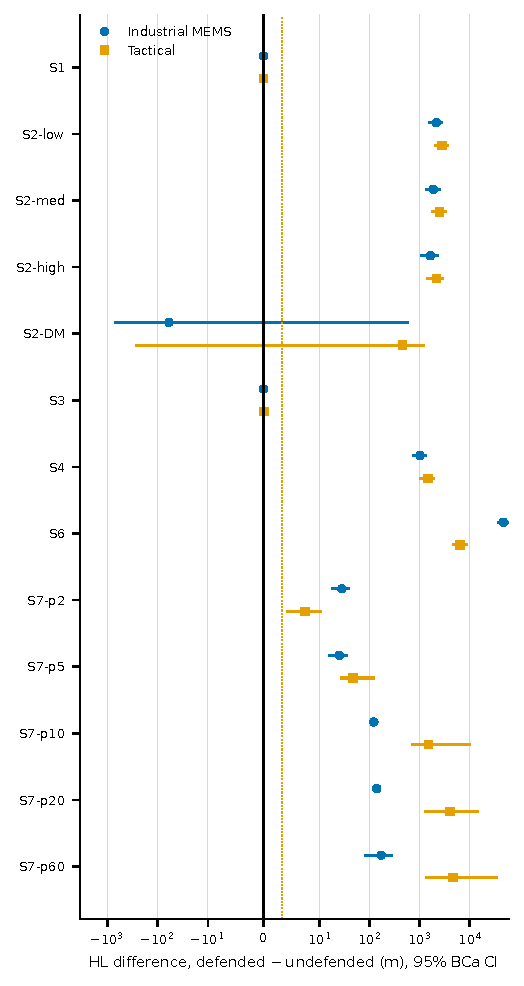
\includegraphics[width=0.8\textwidth]{figures/results_safety_overview.pdf}
\caption{Safety principle: HL difference in maximum horizontal error, defended minus undefended, with $95\%$ BCa CI (symlog axis); dotted lines mark $3\sigma_{\mathrm{nom}}$.}
\label{fig:safety}
\end{figure}

\subsection{Headline comparison}
Tables~\ref{tab:head1} and~\ref{tab:head2} compare FedQPNT (FQ) with the undefended filter (UD) and Baseline~A (BA). The pattern separates cleanly into scenarios in which FedQPNT costs nothing or helps, and scenarios in which it is worse.

\paragraph{Nominal operation and jamming (S1, S3).} FedQPNT is equal to the undefended filter in nominal horizontal error at the MEMS grade ($2.91$ versus $2.90\,\mathrm{m}$) and marginally better at the tactical grade (HL $-0.036\,\mathrm{m}$, CI $[-0.072,-0.006]$); the alarm fraction is $0$ in all arms. Its clock error is marginally worse ($10.4$ versus $10.0\,\mathrm{ns}$). The S1 acceptance criteria pass on horizontal error relative to fixed trust (median ratio $0.997$ MEMS, $0.991$ tactical; bound $1.05$), false alarms ($0$/h), position ANEES ($0.84$ and $0.94$, band $[0.5,2]$) and mean GNSS weight ($0.975$), but the total variation of the GNSS weight ($12.5$ and $12.6$ per hour against a bound of $1$) fails. Under jamming (S3) attack-window error is equal to the undefended and Baseline~A arms at both grades.

\paragraph{Displaced meaconer (S2-DM).} At the MEMS grade the attack-window horizontal error is lower than undefended (median $943$ versus $1{,}340\,\mathrm{m}$; HL $-471\,\mathrm{m}$, CI $[-743,-202]$) and than Baseline~A ($2{,}150\,\mathrm{m}$; HL $-5{,}020\,\mathrm{m}$). At the tactical grade it is indistinguishable from undefended and lower than Baseline~A ($3{,}010\,\mathrm{m}$). Clock error falls from $5{,}220\,\mathrm{ns}$ undefended to $634\,\mathrm{ns}$ (HL $-4{,}570\,\mathrm{ns}$, CI $[-5{,}180,-4{,}180]$), and is also lower than Baseline~A ($1{,}220$ and $2{,}230\,\mathrm{ns}$). The cost is paid after the attack: post-attack horizontal error is higher than both comparators ($1{,}310$ versus $859$ undefended and $268\,\mathrm{m}$ Baseline~A at the MEMS grade), and the alarm fraction is $0.169$ versus $0.021$ undefended and $0.0027$ Baseline~A.

\paragraph{Gradual spoofing (S2).} Here FedQPNT is worse than the undefended filter in the attack window at both grades (medium severity, MEMS: $760$ versus $254\,\mathrm{m}$; tactical: $973$ versus $254\,\mathrm{m}$) and equal to Baseline~A at the MEMS grade for all three severities. Post-attack error is much larger than for either comparator (medium, MEMS: $1{,}120$ versus $189\,\mathrm{m}$ undefended and $5.69\,\mathrm{m}$ Baseline~A), and the alarm fraction is $0.164$ versus $0$. Detection is nevertheless faster than both comparators by $0.5$--$1\,\mathrm{s}$ at all severities and grades.

\paragraph{Jam-then-spoof (S4) and the four-hour drift spoof (S6).} In S4 FedQPNT detects the attack at a median $42\,\mathrm{s}$ against $61\,\mathrm{s}$ for both comparators (HL $-19.5\,\mathrm{s}$), but its attack-window error ($461$ and $638\,\mathrm{m}$) exceeds the undefended filter ($137\,\mathrm{m}$) and Baseline~A. In S6 the attack-window error is $16{,}200\,\mathrm{m}$ (MEMS) and $2{,}680\,\mathrm{m}$ (tactical) against $438\,\mathrm{m}$ undefended, and clock error is $3{,}790$ versus $11.6\,\mathrm{ns}$. Detection is as quick as or quicker than the undefended filter ($1\,\mathrm{s}$ median), but here detection does not translate into lower error.

\begin{table}[ht]
\centering
\caption{Horizontal error RMSE$_h$ (m), median over 30 seeds. FQ: FedQPNT; UD: undefended; BA: Baseline~A. Verdict (B: FQ better; W: worse; $=$: CI includes zero) is FQ against UD/BA. The S1 entry is the nominal-window RMSE$_h$. S6 has no Baseline~A arm.}
\label{tab:head1}
\scriptsize
\setlength{\tabcolsep}{3pt}
\begin{tabular}{llrrrcrrrc}
\toprule
 & & \multicolumn{4}{c}{Attack window} & \multicolumn{4}{c}{Post-attack} \\
\cmidrule(lr){3-6}\cmidrule(lr){7-10}
Scen. & Grade & FQ & UD & BA & vs UD/BA & FQ & UD & BA & vs UD/BA \\
\midrule
S1 & MEMS & 2.91 & 2.9 & 2.9 & =/= & -- & -- & -- & -- \\
 & Tact. & 2.9 & 2.96 & 2.95 & B/B & -- & -- & -- & -- \\
S2-med & MEMS & 760 & 254 & 623 & W/= & 1{,}120 & 189 & 5.69 & W/W \\
 & Tact. & 973 & 254 & 569 & W/W & 1{,}310 & 191 & 5.76 & W/W \\
S2-DM & MEMS & 943 & 1{,}340 & 2{,}150 & B/B & 1{,}310 & 859 & 268 & W/W \\
 & Tact. & 1{,}050 & 1{,}340 & 3{,}010 & =/B & 1{,}420 & 887 & 296 & W/W \\
S3 & MEMS & 14.3 & 14.4 & 14.4 & =/= & 2.58 & 2.6 & 2.6 & B/B \\
 & Tact. & 21.1 & 21.1 & 21.1 & =/= & 2.42 & 2.43 & 2.42 & B/B \\
S4 & MEMS & 461 & 137 & 227 & W/W & 1{,}430 & 165 & 5.45 & W/W \\
 & Tact. & 638 & 137 & 104 & W/W & 1{,}790 & 167 & 5.31 & W/W \\
S6 & MEMS & 16{,}200 & 438 & -- & W/-- & 24{,}600 & 268 & -- & W/-- \\
 & Tact. & 2{,}680 & 438 & -- & W/-- & 3{,}840 & 268 & -- & W/-- \\
\bottomrule
\end{tabular}
\end{table}

\begin{table}[ht]
\centering
\caption{Detection latency (s from onset) and clock error RMSE$_t$ (ns), median over 30 seeds; notation as in Table~\ref{tab:head1}. S1 has no attack, so no latency is defined.}
\label{tab:head2}
\scriptsize
\setlength{\tabcolsep}{3pt}
\begin{tabular}{llrrrcrrrc}
\toprule
 & & \multicolumn{4}{c}{Detection latency} & \multicolumn{4}{c}{Clock RMSE$_t$} \\
\cmidrule(lr){3-6}\cmidrule(lr){7-10}
Scen. & Grade & FQ & UD & BA & vs UD/BA & FQ & UD & BA & vs UD/BA \\
\midrule
S1 & MEMS & -- & -- & -- & -- & 10.4 & 10 & 10 & W/W \\
 & Tact. & -- & -- & -- & -- & 10.4 & 10 & 10 & W/W \\
S2-med & MEMS & 1 & 1 & 1 & B/B & 743 & 10.5 & 412 & W/W \\
 & Tact. & 1 & 1 & 1 & B/B & 743 & 10.5 & 412 & W/W \\
S2-DM & MEMS & 1 & 1 & 1 & =/= & 634 & 5{,}220 & 1{,}220 & B/B \\
 & Tact. & 1 & 1 & 1 & =/= & 634 & 5{,}220 & 2{,}230 & B/B \\
S3 & MEMS & 62 & 62 & 62 & =/= & 29.4 & 29.3 & 29.3 & W/W \\
 & Tact. & 62 & 62 & 62 & =/= & 29.4 & 29.3 & 29.3 & W/W \\
S4 & MEMS & 42 & 61 & 61 & B/B & 748 & 17.3 & 231 & W/W \\
 & Tact. & 42 & 61 & 61 & B/B & 748 & 17.3 & 231 & W/W \\
S6 & MEMS & 1 & 1 & -- & B/-- & 3{,}790 & 11.6 & -- & W/-- \\
 & Tact. & 1 & 1 & -- & B/-- & 3{,}790 & 11.6 & -- & W/-- \\
\bottomrule
\end{tabular}
\end{table}

\begin{figure}[ht]
\centering
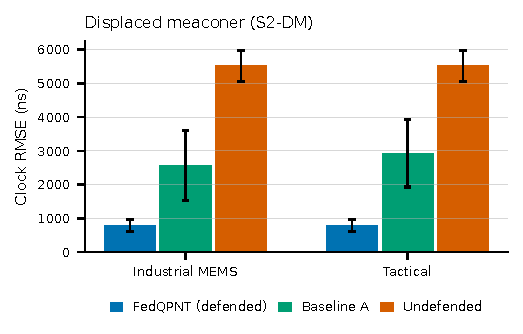
\includegraphics[width=0.85\textwidth]{figures/results_timing_meaconing.pdf}
\caption{Clock RMSE under the displaced meaconer (S2-DM): mean and $95\%$ CI over 30 seeds.}
\label{fig:timing}
\end{figure}

\begin{figure}[ht]
\centering
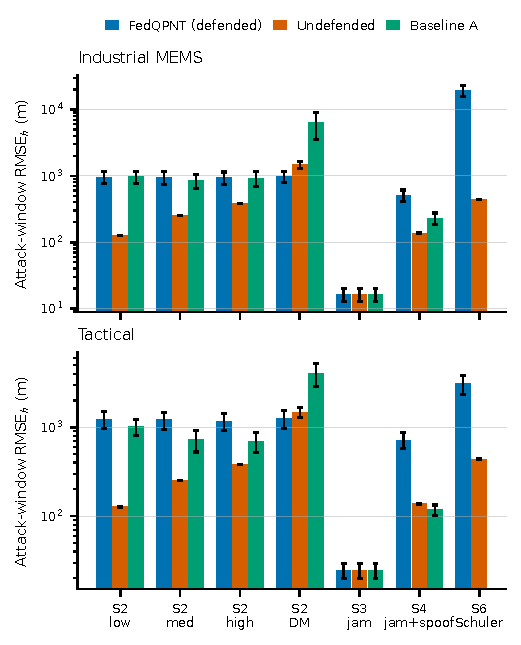
\includegraphics[width=\textwidth]{figures/results_defended_vs_undefended.pdf}
\caption{Attack-window RMSE$_h$ (mean and $95\%$ CI over 30 seeds, log scale) for FedQPNT, the undefended filter and Baseline~A, per scenario and IMU grade.}
\label{fig:defended}
\end{figure}

\subsection{Illustrative single-seed demonstration}
Figure~\ref{fig:demo} shows one live run of the displaced-meaconer scenario (S2-DM, industrial MEMS) on a \emph{tuning} seed (531), with FedQPNT, the undefended filter and Baseline~A. It is an illustration of the mechanism, not evidence: it is a single seed, outside the pre-registered test set, and its numbers differ from the 30-seed medians above. In the run the attack begins at $60\,\mathrm{s}$ and lasts $300\,\mathrm{s}$. The detector flags the signal within about $2\,\mathrm{s}$ and the position trust drops to its floor; the filter then coasts on the inertial and quantum accelerometer. Every roughly $70\,\mathrm{s}$ the engine briefly enters PROBE and rejects the still-fake GNSS; after the attack ends one probe passes and GNSS is re-admitted at $t=411\,\mathrm{s}$, snapping the error back to about a metre. Attack-window RMSE is $592\,\mathrm{m}$ for FedQPNT, $2{,}371\,\mathrm{m}$ undefended and $612\,\mathrm{m}$ for Baseline~A, and clock RMSE is $1{,}652$, $7{,}655$ and $760\,\mathrm{ns}$ respectively. On this seed the simple detect-and-exclude Baseline~A is similar to FedQPNT in position and better in clock error; the clear gain is against the undefended receiver, and the re-admission dwell visibly delays the recovery of FedQPNT relative to Baseline~A (which recovers at about $360\,\mathrm{s}$).

\begin{figure}[ht]
\centering
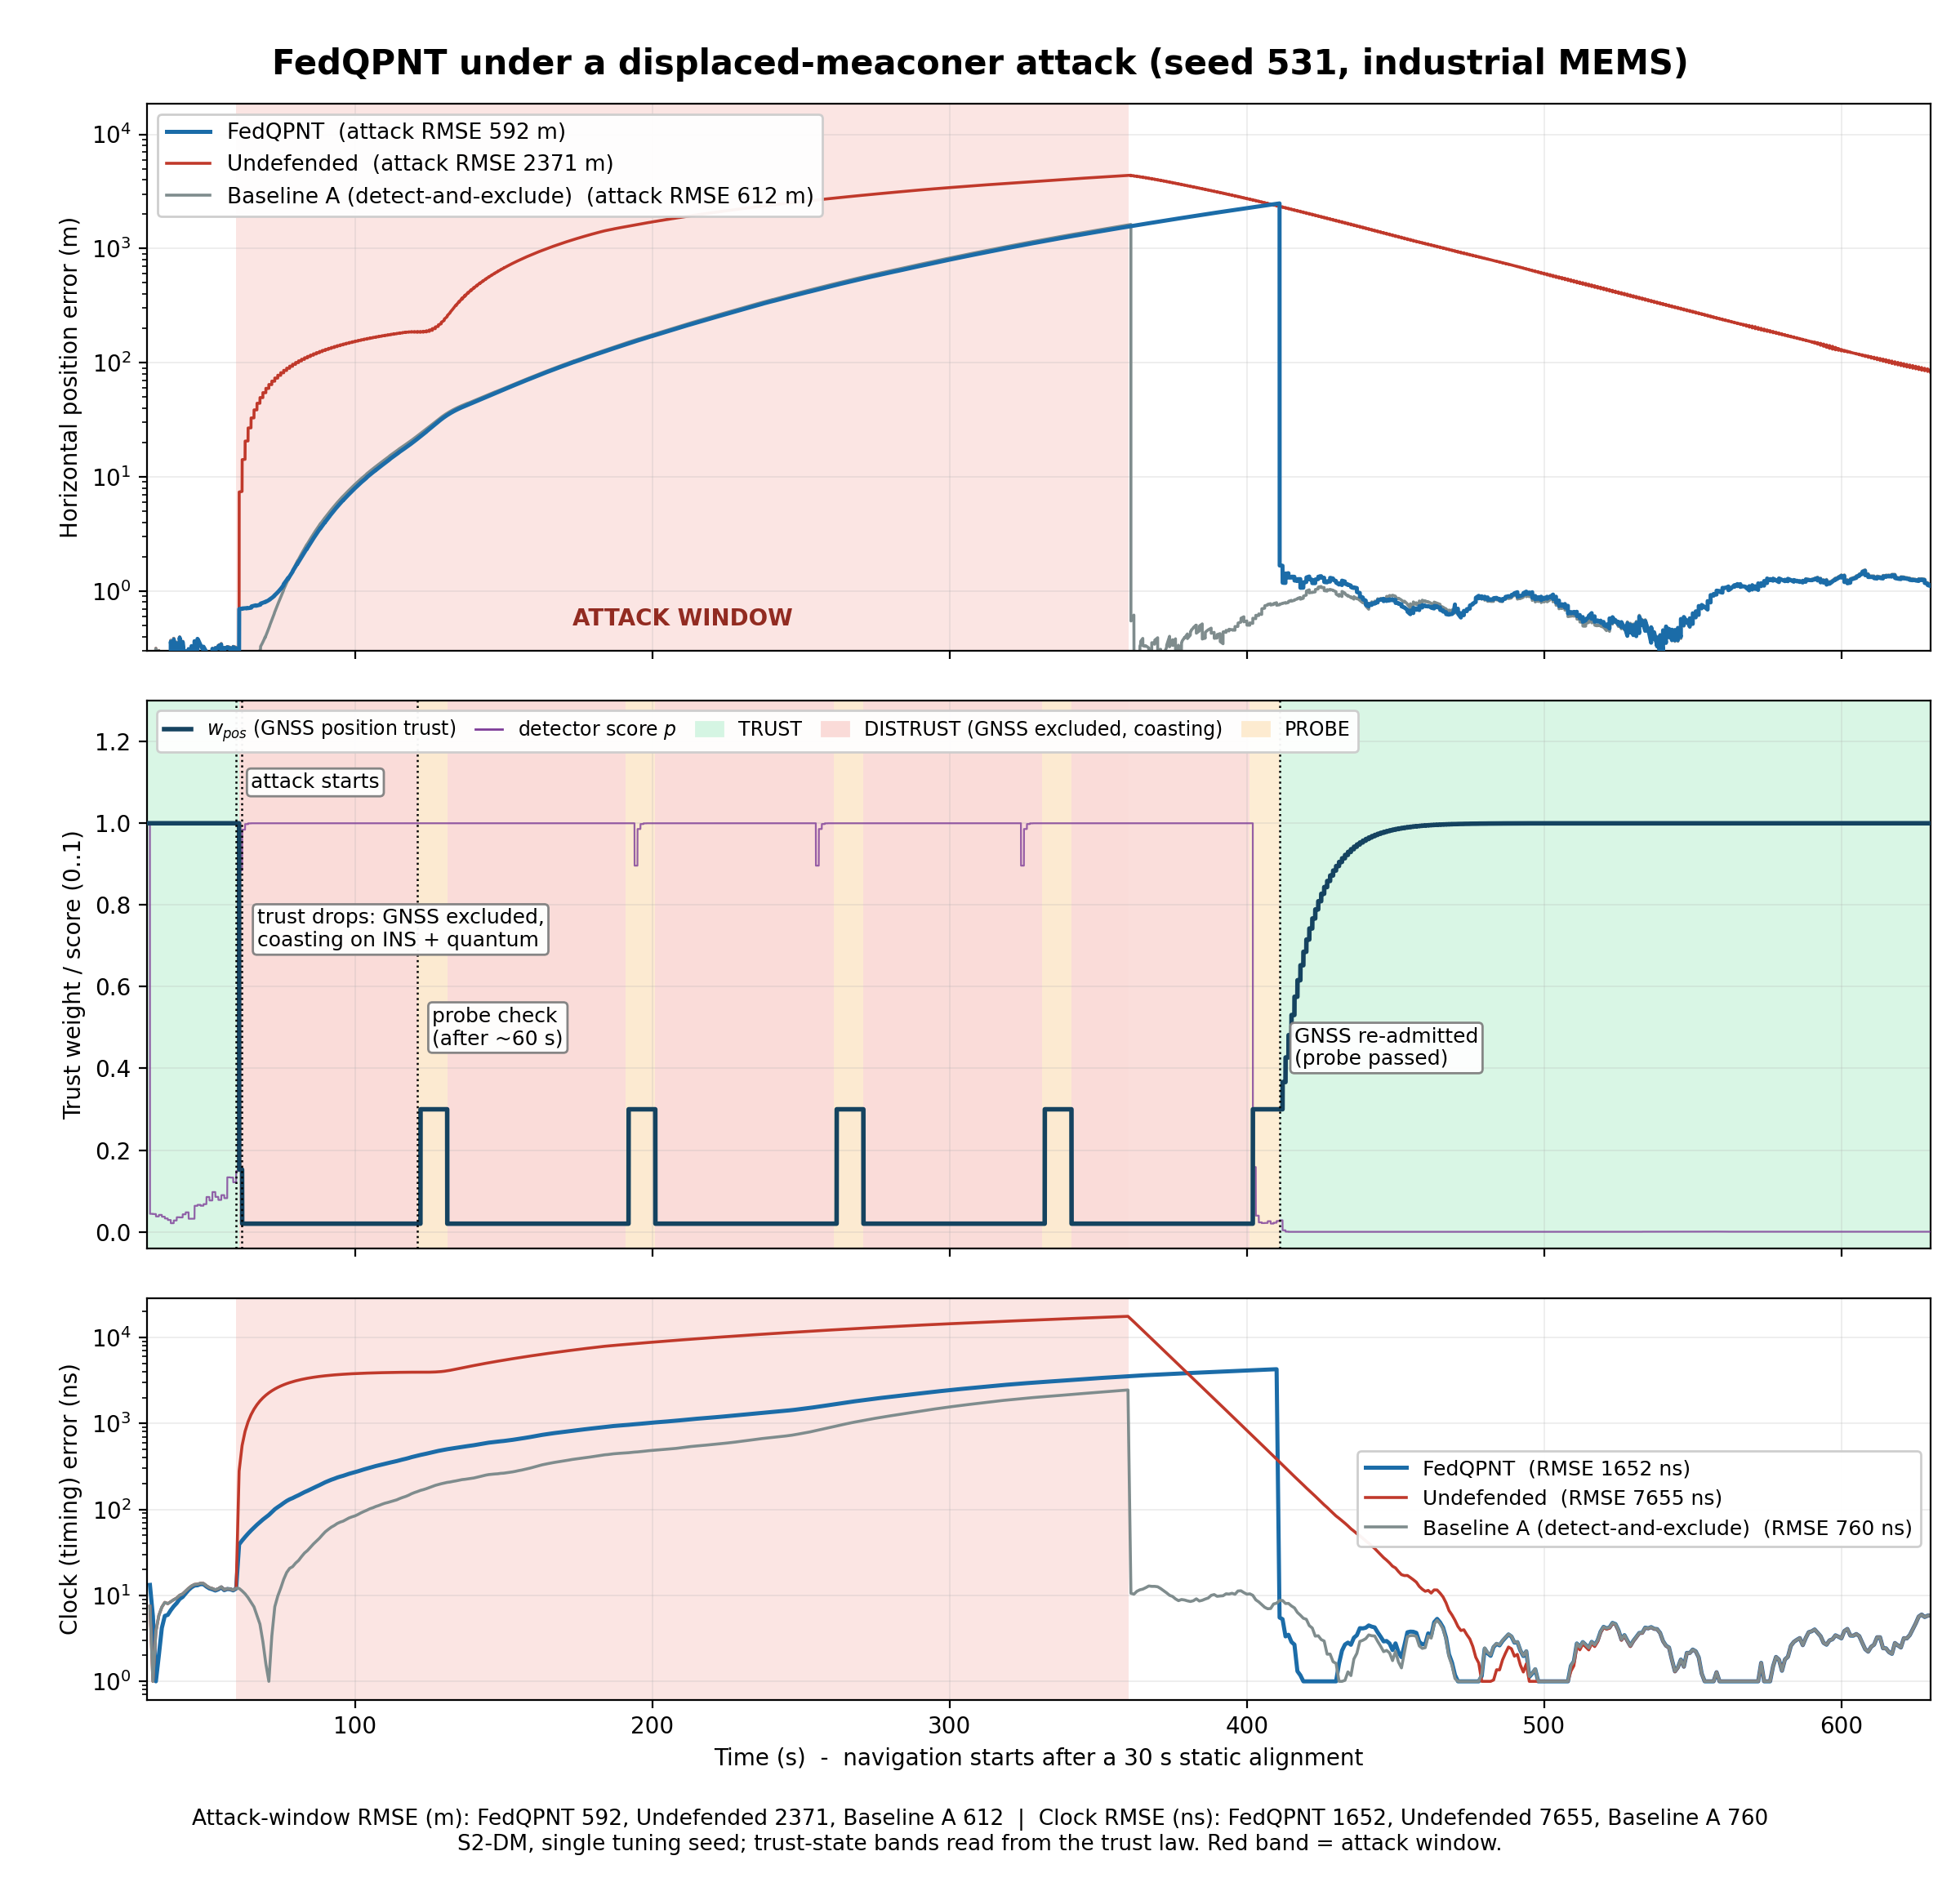
\includegraphics[width=0.92\textwidth]{figures/demo_attack_S2DM.png}
\caption{Single-seed demonstration (tuning seed 531, industrial MEMS, S2-DM): horizontal error (top), FedQPNT trust weight and TRUST/DISTRUST/PROBE state (middle) and clock error (bottom). Illustrative only; not part of the confirmatory evaluation.}
\label{fig:demo}
\end{figure}

\subsection{Trust chattering and long-duration stability}
Across the ten S7 variants (toggle periods $2$ to $60\,\mathrm{s}$, both grades) the maximum number of trust cycles per hour observed in any run was $4$ for $p\le5\,\mathrm{s}$, $1$ for $p=10$ and $20\,\mathrm{s}$, and $29$ (MEMS) and $13$ (tactical) for $p=60\,\mathrm{s}$, all within the proven bound of $223$ per hour (and the $133$ per hour regular-grid figure). Bounded chattering does not imply small error: FedQPNT is worse than undefended on attack-window horizontal error in all S7 variants (Table~\ref{tab:safety}), and on the tactical grade rapid toggling accumulates long exclusion; a pure blackout gives the same result.

In the four-hour nominal mission (S14) the median horizontal RMSE of the last hour is $0.786$ (MEMS) and $0.840$ (tactical) of the first hour (criterion $\le1.2$), i.e.\ there is no slow drift; the median RMSE$_h$ is $2.98\,\mathrm{m}$ and $2.90\,\mathrm{m}$, the alarm fraction is $0$, every run is finite and positive-definite, and the false-alarm rate is $0.067$ per hour (criterion $\le1$). The registry marks S14 ``not evaluable'' overall because its covariance-growth leg is not emitted by the runner.

\subsection{Quantum aiding: a null result}
In the exploratory $180\,\mathrm{s}$ forced-outage test the CAI did not reduce the maximum coasting error (Fig.~\ref{fig:cai}). The median ratio of the maximum error without and with the CAI is $1.006$ at the MEMS grade (mean maximum error $513.4\,\mathrm{m}$ without and $521.4\,\mathrm{m}$ with the CAI; HL CI $[-11.7,20.9]$) and $0.986$ at the tactical grade ($106.1$ versus $104.6\,\mathrm{m}$); the $2.1$--$3.4\times$ envelope seen on tuning seeds was not reproduced. The confirmatory H3 test shows identical effective detection latency with and without the CAI at both grades (Table~\ref{tab:conf}).

\begin{figure}[ht]
\centering
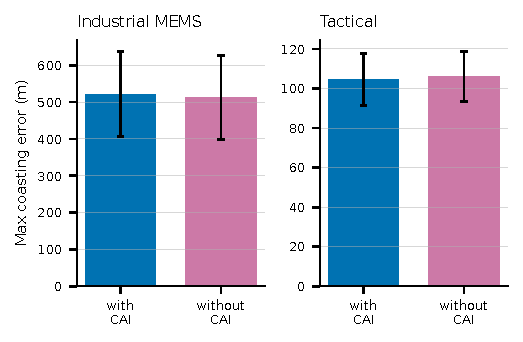
\includegraphics[width=0.8\textwidth]{figures/results_cai_coasting.pdf}
\caption{Maximum horizontal coasting error in a $180\,\mathrm{s}$ GNSS outage with and without the CAI: mean and $95\%$ CI over 30 seeds, per IMU grade.}
\label{fig:cai}
\end{figure}

\subsection{Fleet experiments and federated learning: a null result}
\label{sec:res-fleet}
\paragraph{Functional federation.} Fleet nodes install the global model: in the abrupt H2 experiment FedQPNT nodes installed it in $9.6$ of $10$ rounds on average, against $8.0$ for B-cont. In S5 (node failures and delayed updates) no run deadlocked or aborted and $5.93$ rounds per run were gracefully skipped; in S8 a cold-start node received the global model within two rounds of joining in every run. In S15 (simultaneous attack on $30\%$ of a ten-node fleet) the detection probability over attacked nodes is $1.000$, the attacked-node attack-window error is $935\pm115\,\mathrm{m}$ (mean, $95\%$ CI), the false-alarm rate on unattacked nodes is $0$ per hour, and no quarantine occurred. The clean-window error and alarm rate in S12 (sign-flip poisoning at $f=20\%$ and $40\%$) are identical to the clean-fleet arm ($2.79\pm0.14\,\mathrm{m}$, $0$ false alarms per hour). The AUC-based legs of S5, S9 and S12 are undefined because those scenarios contain no attack, so the poisoning robustness of TRIM-NB-R against FedAvg is \emph{not} evaluated in this round.

\paragraph{H2 and H4 (abrupt spoof, $n=10$).} At the pre-registered per-arm threshold both FedQPNT and B-cont detect every event at the onset epoch ($P_D@10\,\mathrm{s}=1$, latency $0\,\mathrm{s}$, no censored events), so the paired tests are degenerate. The secondary onset-window AUC is near chance for both arms: H2, $0.505$ versus $0.507$; H4, $0.526$ versus $0.501$ (uncorrected paired $p=0.006$, exploratory, outside the Holm family). Per-seed values range from $0.20$ to $0.89$ in both arms (Fig.~\ref{fig:h2h4}), and the H4 mean difference of $+0.025$ is small against that spread; we do not interpret it as a detection benefit.

\begin{figure}[ht]
\centering
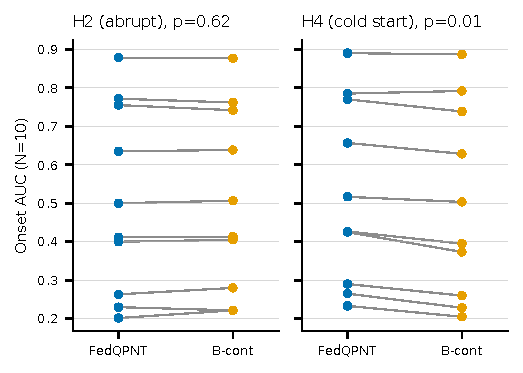
\includegraphics[width=0.8\textwidth]{figures/results_h2h4_auc_paired.pdf}
\caption{Per-seed onset-window AUC ($N=10\,\mathrm{s}$), FedQPNT versus B-cont, for H2 and H4 ($n=10$ seeds each); $p$ is the uncorrected paired Wilcoxon value.}
\label{fig:h2h4}
\end{figure}

\subsection{Other scenarios}
For the sample-rate-mismatch scenarios (S10) the position ANEES lies in the band $[0.5,2]$ at GNSS rates of $1$ and $2\,\mathrm{Hz}$ and outside it at $5\,\mathrm{Hz}$ ($3.26$--$3.47$) and $10\,\mathrm{Hz}$ ($6.40$--$6.62$). In the extreme-noise scenario (S11) the filter locks out GNSS, so its error is far above raw GNSS (median ratio $5{,}494$ MEMS, $1{,}823$ tactical; criterion $\le1.5$). In the recovery scenario (S13) no run recovers within $60\,\mathrm{s}$ at either grade; at the MEMS grade $20$ of $30$ runs recover within $180\,\mathrm{s}$ and at the tactical grade none do, so the pre-registered recovery bounds fail.

\subsection{Discussion}
\paragraph{When trust-based exclusion pays.} The measured benefits are concentrated where excluding GNSS removes a large, sustained error. Against the displaced meaconer FedQPNT lowers attack-window horizontal error relative to Baseline~A at both grades and relative to the undefended filter at the MEMS grade, and reduces median clock error about eight-fold ($634$ versus $5{,}220\,\mathrm{ns}$). It detects attack onset earlier than a binary detect-and-exclude baseline (by $0.5$ to $1\,\mathrm{s}$ in gradual-spoof scenarios and by $19.5\,\mathrm{s}$ in jam-then-spoof), at no cost in nominal operation or under jamming; trust cycles at most $29$ times per hour against a proven bound of $223$, and a four-hour mission shows no drift.

\paragraph{When it does not.} Against ordinary drifting spoofs (S2) and the jam-then-spoof, long-drift and toggling scenarios (S4, S6, S7), FedQPNT's horizontal error is larger than that of the undefended filter, so the safety principle fails. Two mechanisms are consistent with this. First, when the spoof offset is small the inertial coast drifts further than the spoof displaces the position: at the MEMS grade the undefended filter that simply follows the spoof ($127$ to $381\,\mathrm{m}$ across S2 severities) is below the coast error of an excluding filter ($730$ to $770\,\mathrm{m}$). Second, post-attack error is dominated by the designed $60\,\mathrm{s}$ re-admission dwell. The tactical grade should coast better yet is not better here, so the coast floor alone does not explain the loss; a plausible but untested contributor is residual over-confidence of the attitude and accelerometer-bias states during long coasts. We read the results as characterising the regime in which exclusion pays rather than as a uniform improvement over not defending.

\paragraph{CAI and federated learning showed no measurable effect here.} Three untested hypotheses are offered. (i) The rigid-mode CAI loses contrast above $\Omega_c\approx17\,\mathrm{mrad/s}$, so its aiding is intermittent in manoeuvring motion, and its bias observation may add little to a filter whose coast error is dominated by tilt. (ii) The rule-based physical evidence, not the learned detector, may drive detection at the tested severities, making latency insensitive to both the CAI and the federated model; the primary metric is at its ceiling, so a harder setting is needed to separate the arms. (iii) The experiments are simulation-only and use ten live seeds for the fleet tests. The null results are results about this configuration; they are not evidence that quantum aiding or fleet learning cannot help.

%=====================================================================
\section{Conclusions}
\label{sec:conclusion}
%=====================================================================

\subsection{Summary}
We have presented FedQPNT, a system architecture that closes the loop between a learned, fleet-shared attack detector, a continuous and evidence-bounded per-sensor trust law, and physical quantum inertial aiding whose noise and fault behaviour is calibrated against real laboratory data, and we have evaluated it in a pre-registered round of $5{,}340$ simulated runs on unseen seeds. The evidence supports a specific and bounded set of conclusions. The continuous trust law detects attack onset significantly earlier than a detect-and-exclude baseline (median $0.5\,\mathrm{s}$, Holm-adjusted $p=0.004$), adds no measurable cost in nominal operation or under jamming, cycles trust at most $29$ times per hour against a proven bound of $223$, remains stable over four hours, and, against a displaced meaconer, lowers attack-window horizontal error relative to the baseline and cuts median clock error about eight-fold.

The study did \emph{not} show that the cold-atom accelerometer improves coasting or detection (coasting-error ratio $1.006$ and $0.986$; H3 null), that federated learning improves abrupt-spoof detection (H2 and H4 null, with the primary metric at its ceiling), or that FedQPNT reduces position error under ordinary drifting spoofs, where its error exceeded that of the undefended filter at both IMU grades and the safety principle failed; the position-error component of H1 was not significant. These outcomes delimit the regime in which GNSS exclusion pays: large or timing-corrupting offsets.

\subsection{Limitations}
\begin{itemize}
\item \textbf{No position benefit under ordinary spoofing.} In S2, S4, S6 and S7 the attack-window error exceeds that of the undefended filter at both grades; post-attack error is raised by the $60\,\mathrm{s}$ re-admission dwell.
\item \textbf{No measured benefit from the CAI or from federated learning}; single-node results involve no federation, the fleet tests use $n=10$ seeds, and TRIM-NB-R's robustness against FedAvg was not evaluated.
\item \textbf{Signature-strength envelope.} Detection of a drifting single-antenna spoofer relies on its C/N0 signature strength $s\gtrsim0.5$, an explicit operating assumption; a signature-free multi-antenna spoofer is outside the threat model, and the sweep was not run in the round-3 campaign.
\item \textbf{A consistency-matched adversary can pass the shadow probe.} An offset kept inside the coasting uncertainty is consistent with the coasting state; the bound is looser at the MEMS grade.
\item \textbf{Clock-only evidence is weak just after a long outage}, since the oscillator uncertainty is large (about $263\,\mathrm{m}$ after $180\,\mathrm{s}$; a $750\,\mathrm{m}$ replay step is only about $2.9\sigma$).
\item \textbf{The filter may remain over-confident in attitude and accelerometer bias.} The round-3 campaign measured position ANEES only ($0.84$ and $0.94$); the earlier bias-NEES figure (about six times nominal on tuning seeds) was not re-measured.
\item \textbf{Simulation-only evaluation.} Only the CAI noise model is calibrated to real laboratory data; trajectories, GNSS signals, receiver and clock are simulated, and the truth clock shares the filter's model, so timing results are model-consistent by construction.
\item \textbf{Rigid-mode quantum aiding is intermittent in manoeuvres}, with a rotation-rate tolerance of about $17\,\mathrm{mrad/s}$ against about $0.3\,\mathrm{rad/s}$ in an ordinary vehicle turn.
\item \textbf{Scoped novelty.} G\textsuperscript{2}FL \cite{liu2026g2fl} already provides robust FL for GNSS spoofing; the contribution is the closed loop of FL detector, continuous bounded trust and quantum aiding, not robust aggregation alone.
\end{itemize}

\subsection{Future work}
The results point to four directions: (i) harder detection settings (lower-severity or signature-free families, stricter latency metrics) that can separate the federated and local arms, together with an AUC-based poisoning comparison of TRIM-NB-R against FedAvg; (ii) filter consistency during long coasts, including re-measuring attitude and bias NEES and a coupled or tightly coupled formulation, which bears on both the coast error and the unexplained tactical-grade result; (iii) shortening or adapting the re-admission dwell, to reduce post-attack error without losing the evidence-bounded property; and (iv) a quantum sensor mode that tolerates vehicle rotation rates (inertial-pointing), and ultimately a real-data or hardware-in-the-loop evaluation.

\bibliographystyle{plain}
\bibliography{refs}
\addcontentsline{toc}{section}{References}

\end{document}
